Use the six observations on the variable $X_1$ in units of millions, from Table 1.1.
\begin{enumerate}[label=(\alph*)]
    \item Find the projection on $\textbf{1}^{\prime}=[1,1,1,1,1,1]$.
    \par
    Convert $X_1$ to units of millions
    \[
        \textbf{y}_1
        =
        \left(\frac{1}{1000000}\right)
        \begin{bNiceArray}{c}
            3497900 \\
            2485475 \\
            1782875 \\
            1725450 \\
            1645575 \\
            1469800
        \end{bNiceArray}
        =
        \begin{bNiceArray}{c}
            3.4979 \\
            2.4855 \\
            1.7829 \\
            1.7254 \\
            1.6456 \\
            1.4698
        \end{bNiceArray}
    \]
    \[
        \text{Proj}_{\textbf{1}_6}{\textbf{y}_1}
        =
        \left(\frac{\textbf{1}_6 \cdot \textbf{y}_1}{\left\|\textbf{1}_6\right\|}\right)\frac{\textbf{1}_6}{\left\|\textbf{1}_6\right\|}
        =
        \bar{x}_1 \textbf{1}_6
        =
        2.1012
        \begin{bNiceArray}{c}
            1 \\
            1 \\
            1 \\
            1 \\
            1 \\
            1
        \end{bNiceArray}
        =
        \begin{bNiceArray}{c}
            2.1012 \\
            2.1012 \\
            2.1012 \\
            2.1012 \\
            2.1012 \\
            2.1012
        \end{bNiceArray}
    \]
    \item Calculate the deviation vectot $\textbf{y}_1 - \bar{x}_1\textbf{1}$. Relate its length to the sample standard deviation.
    \[
        \textbf{y}_1 - \bar{x}_1\textbf{1}
        =
        \begin{bNiceArray}{c}
            3.4979 \\
            2.4855 \\
            1.7829 \\
            1.7254 \\
            1.6456 \\
            1.4698
        \end{bNiceArray}
        -
        \begin{bNiceArray}{c}
            2.1012 \\
            2.1012 \\
            2.1012 \\
            2.1012 \\
            2.1012 \\
            2.1012
        \end{bNiceArray}
        =
        \begin{bNiceArray}{r}
            1.3967 \\
            0.3843 \\
            -0.3183 \\
            -0.3757 \\
            -0.4556 \\
            -0.6314
        \end{bNiceArray}
    \]
    The sample variance for the first variable (feature, predictor, or whatever) is
    \[
        \sqrt{s_{11}}
        =
        \sqrt{\frac{\sum_{i=1}^{6}{{(x_{i1}- \bar{x}_1)}^2}}{n-1}}
        =
        \sqrt{\frac{{(\textbf{y}_1 - \bar{x}_1\textbf{1})}^{\prime}(\textbf{y}_1 - \bar{x}_1\textbf{1})}{n-1}}
        =
        \frac{\left\|\textbf{y}_1 - \bar{x}_1\textbf{1}\right\|}{\sqrt{n-1}}
    \]
    \[
        \Rightarrow
        \left\|\textbf{y}_1 - \bar{x}_1\textbf{1}\right\|
        =
        \sqrt{s_{11}}\sqrt{n-1}
    \]
    The length of $\textbf{y}_1 - \bar{x}_1\textbf{1}$ is the sample standard deviation times the square root of $n-1$.
    For our data, $\left\|\textbf{y}_1 - \bar{x}_1\textbf{1}\right\| = 1.7167$.

    \item Graph (to scale) the triangle formed by $\textbf{y}_1$, $\bar{x}_1\textbf{1}$, and $\textbf{y}_1 - \bar{x}_1\textbf{1}$. Identify the length of each component on your graph.
    \begin{figure}[H]
        \centering
        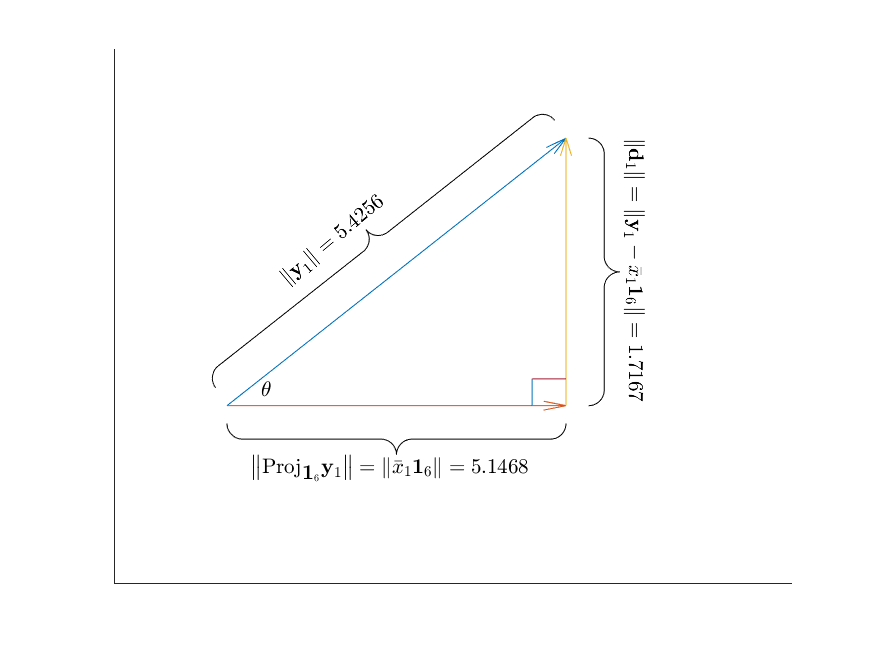
\includegraphics[scale=0.5]{./matlab/chapter-3/sol3.4c.png}
    \end{figure}

    \begin{lstlisting}
        % Divide original units by 1,000,000 so we're in units of millions.
y1 = [3497900 2485475 1782875 1725450 1645575 1469800]'/1000000;
a1 = ones(height(y1),1);
% The projection of y1 onto a1.
x1bar1 = ((y1'*a1)/(norm(a1)*norm(a1)))*a1;

% Exercise 3.4 (b)
d1 = y1 - x1bar1;

% Exercise 3.4 (c)
clear clf
hold on
start = zeros(1,2);
quiver(start(:,1), start(:,2), 1, 1, 3);
quiver(start(:,1), start(:,2), 1, 0, 3);
quiver(3, 0, 0, 1, 3);
xlim([-1,5])
ylim([-2,4])
% Use the DRAWBRACE created by Pal Naverlid Savik
drawbrace([3.2, -0], [3.2, -3],10,1,'Color','k') % Draws a curly brace for deviance vector.
% Text for the norm of deviance vector d1, norm(d1).
anno = join(["$$\left\|\textbf{d}_1\right\|"," = \left\|\textbf{y}_1 - \bar{x}_1 \textbf{1}_6 \right\| = 1.7167$$"],'');
text(3.2+0.4,1.5+1.5,anno,'Rotation',270,'interpreter','latex');

drawbrace([0, 0.2], [3, 0.2],10,1,'Color','k') % Draws a curly brace for projection vector
% % Text for the norm of the projection vector, norm(x1bar1).
anno = join(["$$\left\|\rm{Proj}_{\textbf{1}_6}\textbf{y}_1 \right\| = \left\|\bar{x}_1\textbf{1}_6\right\|"," = 5.1468$$"],'');
text(0.2,-0.7,anno,'interpreter','latex');

drawbrace([-0.1, 0.2], [2.9, 3.2],10,0,'Color','k') % Draws a curly brace for y vector.
% Text for the norm of y2, norm(y1).
anno = join(["$$\left\|\textbf{y}_1 \right\| = "," 5.4256$$"],'');
text(0.5,1.4,anno,'Rotation',40,'interpreter','latex');

% Include text for angle theta.
text(0.3,0.2,'\theta')

% Include the right-angle symbol on plot.
plot([3,2.7],[0.3,0.3])
plot([2.7,2.7],[0,0.3])
set(gca,'xtick',[],'ytick',[]);
hold off
saveas(gcf,'sol3.4c.png')
    \end{lstlisting}
    \item Repeat Parts a-c for the variable $X_2$ in Table 1.1.
    \[
        \textbf{y}_2
        =
        \begin{bNiceArray}{c}
            0.623 \\
            0.593 \\
            0.512 \\
            0.500 \\
            0.463 \\
            0.395
        \end{bNiceArray}
    \]
    \[
        \text{Proj}_{\textbf{1}_6}{\textbf{y}_2}
        =
        \left(\frac{\textbf{1}_6 \cdot \textbf{y}_2}{\left\|\textbf{1}_6\right\|}\right)\frac{\textbf{1}_6}{\left\|\textbf{1}_6\right\|}
        =
        \bar{x}_2 \textbf{1}_6
        =
        0.5143
        \begin{bNiceArray}{c}
            1 \\
            1 \\
            1 \\
            1 \\
            1 \\
            1
        \end{bNiceArray}
        =
        \begin{bNiceArray}{c}
            0.5143 \\
            0.5143 \\
            0.5143 \\
            0.5143 \\
            0.5143 \\
            0.5143
        \end{bNiceArray}
    \]
    \[
        \textbf{y}_2 - \bar{x}_2\textbf{1}
        =
        \begin{bNiceArray}{c}
            0.623 \\
            0.593 \\
            0.512 \\
            0.500 \\
            0.463 \\
            0.395
        \end{bNiceArray}
        -
        \begin{bNiceArray}{c}
            0.5143 \\
            0.5143 \\
            0.5143 \\
            0.5143 \\
            0.5143 \\
            0.5143
        \end{bNiceArray}
        =
        \begin{bNiceArray}{r}
            1.3967 \\
            0.3843 \\
            -0.3183 \\
            -0.3757 \\
            -0.4556 \\
            -0.6314
        \end{bNiceArray}
    \]
    For our data, $\left\|\textbf{y}_2 - \bar{x}_2\textbf{1}\right\| = 0.1873$.
    \begin{figure}[H]
        \centering
        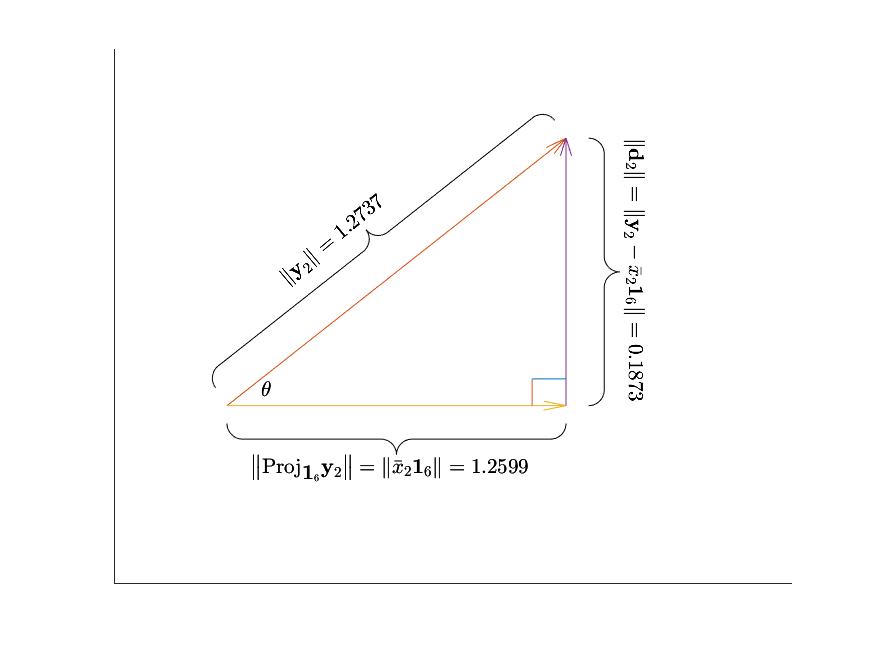
\includegraphics[scale=0.5]{./matlab/chapter-3/sol3.4d.png}
    \end{figure}
    \begin{lstlisting}
        y2 = [0.623 0.593 0.512 0.500 0.463 0.395]';
        % The projection of y2 onto a1.
        x2bar1 = ((y2'*a1)/(norm(a1)*norm(a1)))*a1;
        
        % Compute the deviance vector for y2.
        d2 = y2 - x2bar1;
        
        clear clf
        hold on
        start = zeros(1,2);
        quiver(start(:,1), start(:,2), 1, 1, 3);
        quiver(start(:,1), start(:,2), 1, 0, 3);
        quiver(3, 0, 0, 1, 3);
        xlim([-1,5])
        ylim([-2,4])
        % Use the DRAWBRACE created by Pal Naverlid Savik
        drawbrace([3.2, -0], [3.2, -3],10,1,'Color','k') % Draws a curly brace for deviance vector.
        % Text for the norm of deviance vector d2, norm(d2).
        anno = join(["$$\left\|\textbf{d}_2\right\|"," = \left\|\textbf{y}_2 - \bar{x}_2 \textbf{1}_6 \right\| = 0.1873$$"],'');
        text(3.2+0.4,1.5+1.5,anno,'Rotation',270,'interpreter','latex');
        
        drawbrace([0, 0.2], [3, 0.2],10,1,'Color','k') % Draws a curly brace for projection vector.
        % Text for the norm of the projection vector, norm(x2bar1).
        anno = join(["$$\left\|\rm{Proj}_{\textbf{1}_6}\textbf{y}_2 \right\| = \left\|\bar{x}_2\textbf{1}_6\right\|"," = 1.2599$$"],'');
        text(0.2,-0.7,anno,'interpreter','latex');
        
        drawbrace([-0.1, 0.2], [2.9, 3.2],10,0,'Color','k') % Draws a curly brace for y vector.
        % Text for the norm of y2, norm(y2).
        anno = join(["$$\left\|\textbf{y}_2 \right\| = "," 1.2737$$"],'');
        text(0.5,1.4,anno,'Rotation',40,'interpreter','latex');
        
        % Include text for angle theta.
        text(0.3,0.2,'\theta')
        
        % Include the right-angle symbol on plot.
        plot([3,2.7],[0.3,0.3])
        plot([2.7,2.7],[0,0.3])
        set(gca,'xtick',[],'ytick',[]);
        hold off
        saveas(gcf,'sol3.4d.png')
    \end{lstlisting}
    \item Graph (to scale) the two deviation vectors $\textbf{y}_1 - \bar{x}_1\textbf{1}$ and $\textbf{y}_2 - \bar{x}_2\textbf{1}$. Calculate the value of the angle between them.
    \par
    The deviation vectors are in $\R^6$, so plotting that isn't feasible so here's the plot of the first 3 dimensions.

    \begin{figure}[H]
        \centering
        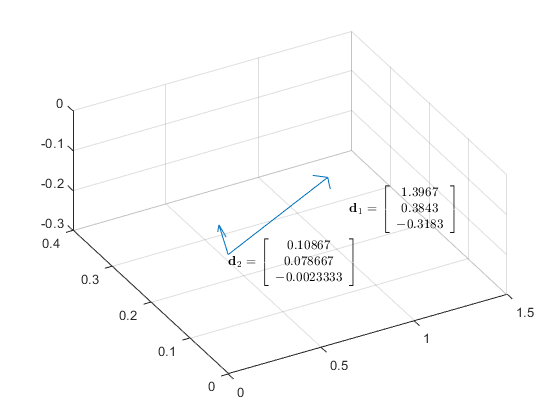
\includegraphics[scale=0.5]{./matlab/chapter-3/sol3.4e.png}
    \end{figure}

    \[
        \cos\theta
        =
        \frac{\textbf{d}_1 \cdot \textbf{d}_2}{\left\|\textbf{d}_1\right\|\left\|\textbf{d}_2\right\|}
        =
        \frac{1}{1.7167 \times 0.1873}
        {
        \begin{bNiceArray}{r}
            1.3967 \\
            0.3843 \\
            -0.3183 \\
            -0.3757 \\
            -0.4556 \\
            -0.6314
        \end{bNiceArray}
        }^{\prime}
        \begin{bNiceArray}{r}
            1.3967 \\
            0.3843 \\
            -0.3183 \\
            -0.3757 \\
            -0.4556 \\
            -0.6314
        \end{bNiceArray}
        = 0.8921
    \]
    \[
        \Rightarrow
        \theta
        =
        {\cos}^{-1}\left(0.8921\right)
        =
        26.8583\degree
    \]

    Also could do
    \[
        \cos\theta
        =
        \frac{\textbf{d}_1 \cdot \textbf{d}_2}{\left\|\textbf{d}_1\right\|\left\|\textbf{d}_2\right\|}
        =
        \frac{(n-1)s_{12}}{\sqrt{(n-1)s_{11}}\sqrt{(n-1)s_{22}}}
        =
        \frac{s_{12}}{\sqrt{s_{11}}\sqrt{s_{22}}}
        =
        r_{12}
    \]
    \[
        \Rightarrow
        \theta = {\cos}^{-1} r_{12} = {\cos}^{-1} (0.8921) = 26.8583\degree
    \]
    \begin{lstlisting}
% Combine the deviation vectors.
D = [d1 d2]';
start = zeros(size(D));

clear clf
% Plot the d_1, d_2 deviation vectors.
quiver3(start(:,1), start(:,2), start(:,3), D(:,1), D(:,2), D(:,3));
% Text for data.
for r = 1:height(D)
    % Labels for the deviation vectors, d_1 and d_2.
    anno = join(["$$\textbf{d}_",r," = \left[\begin{array}{c}",D(r,1),"\\",D(r,2),"\\",D(r,3),"\end{array}\right]$$"],'');
    text(D(r,1)-0.05,D(r,2)-0.05,D(r,3)-0.05,anno,'interpreter','latex');
end

% Compute the angle between d1 and d2.
acosd(d1'*d2/(norm(d1)*norm(d2)))
% Same answer using (2-36) on page 72, R = V^{-1/2} \Sigma V^{-1/2}.
acosd(diag(sqrt(inv(diag(diag(cov(y1,y2)))))*cov(y1,y2)*sqrt(inv(diag(diag(cov(y1,y2))))),1))
    \end{lstlisting}
\end{enumerate}